\chapter{Unintentional Genomic Changes Endow \textit{Cupriavidus metallidurans} with an Augmented Heavy-Metal Resistance }

\section{Foreword}

While looking into the diverse abilities present in the genome of \textit{Cupriavidus metallidurans}, it was observed that mutants of this bacteria are difficult to make or too unstable. A natural plasmid pTP6 was previously introduced into strain CH34, increasing its resistance to mercury. However, resistance to some other heavy metals were also increased but with no direct relation to the resistance markers introduced. After genomic sequencing, it was observed that this bacteria has an inherit genetic unstability allowing it to adapt under harsh conditions. 

The present chapter has been published as a research article entitled “Unintentional Genomic Changes Endow \textit{Cupriavidus metallidurans} with an Augmented Heavy-Metal Resistance” in the peer-reviewed journal Genes. Sections from 4.2 to 4.9 show the published manuscript including its Supplementary Information. Additional information, official links and repositories are mentioned within the chapter text. 

\section{Abstract}

For the past three decades, \textit{Cupriavidus metallidurans} has been one of the major model organisms for bacterial tolerance to heavy metals. Its type strain CH34 contains at least 24 gene clusters distributed over four replicons, allowing for intricate and multilayered metal responses. To gain organic mercury resistance in CH34, broad-spectrum \textit{mer} genes were introduced in a previous work via conjugation of the IncP-1$\beta$ plasmid pTP6. However, we recently noted that this CH34-derived strain, MSR33, unexpectedly showed an increased resistance to other metals (i.e., Co$^{2+}$, Ni$^{2+}$, and Cd$^{2+}$). To thoroughly investigate this phenomenon, we resequenced the entire genome of MSR33 and compared its DNA sequence and basal gene expression profile to those of its parental strain CH34. Genome comparison identified 11 insertions or deletions (INDELs) and nine single nucleotide polymorphisms (SNPs), whereas transcriptomic analysis displayed 107 differentially expressed genes. Sequence data implicated the transposition of IS1088 in higher Co$^{2+}$ and Ni$^{2+}$ resistances and altered gene expression, although the precise mechanisms of the augmented Cd$^{2+}$ resistance in MSR33 remains elusive. Our work indicates that conjugation procedures involving large complex genomes and extensive mobilomes may pose a considerable risk toward the introduction of unwanted, undocumented genetic changes. Special efforts are needed for the applied use and further development of small nonconjugative broad-host plasmid vectors, ideally involving CRISPR-related and advanced biosynthetic technologies.

\section{Introduction}

Since life appeared on earth some 3.7 billion years ago, microorganisms have undergone molecular changes to adapt (i.e., respond to selection) to the harsh conditions of their natural habitats, including extreme temperatures, pH, salinity, UV and ionizing radiation, and heavy metals \citep{bakermans2015microbial}. In addition, global fluctuations in the composition of the atmosphere, the oceans, and the earth crust have elicited genomic changes in microbes over eons of time and hence contributed to microbial diversity \citep{knoll2015paleobiological}. Certain microorganisms had been adapted to heavy metals and radionuclides prior to human appearance. However, during the past few hundred years, anthropogenic influences have forced microbes to also adapt to pollutants previously nonexistent (xenobiotics) \citep{springael2004horizontal, cao2012characterization, ilori2015catabolic, mergeay2014adaptation}, as well as to increased concentrations of heavy metals and radionuclides \citep{nies1999microbial, mergeay2000bacteria, sobecky2009horizontal}.
Members of the \textit{beta}-proteobacterial genus \textit{Cupriavidus} are prime examples of microbial endurance, possessing a variety of genomic islands involved in the resistance to heavy metals or the degradation of aromatics or xenobiotics \citep{pohlmann2006genome, amadou2008genome, janssen2010complete, lykidis2010complete, poehlein2011complete,cserhati2012novo, hong2012whole, li2013genome, ray2015complete, wang2015genome, fang2016complete}. They all typically display a bipartite chromosomal structure with one chromosomal replicon bearing the marks of a plasmid-type maintenance and replication system henceforth called “chromid”. In addition, most \textit{Cupriavidus} strains carry one or two dispensable megaplasmids with a size of 100 kb or more. The model organism for heavy metal resistance, \textit{Cupriavidus metallidurans} strain CH34, carries two megaplasmids, pMOL28 and pMOL30. Together, the four CH34 replicons encode resistance markers for a plethora of heavy metals including copper, nickel, zinc, cobalt, cadmium, chrome, lead, silver, gold, mercury, caesium, selenium, strontium, and uranium \citep{janssen2010complete, mergeay2003ralstonia, monchy2007plasmids, avoscan2007uranium, monsieurs2011heavy, salem2013strontium}. These resistances are mainly related to a variety of metal reduction and efflux systems \citep{van2015genomic, vandenbussche2015metal,nies2016biological}. Aromatics degradation, on the other hand, is carried out by various bacterial multicomponent mono- and di-oxygenases solely encoded by genes on the chromosome and chromid \citep{millacura2017degradation}.
In an effort to improve the inorganic and organic mercury resistance of \textit{C. metallidurans} CH34 and thus improve its utility in cleaning up mercury-contaminated environments, the IncP-1$\beta$ plasmid pTP6, providing additional \textit{mer} genes \citep{smalla2006increased}, was introduced in CH34 by biparental mating, leading to strain MSR33 \citep{rojas2011characterization}. These extra \textit{mer} genes are part of a transposon, Tn50580, which is necessary for broad-spectrum (organomercury) resistance, including two genes, \textit{merG} and \textit{merB}, not native to CH34 (i.e., CH34 only contains two narrow-spectrum mercury resistance \textit{merRTPADE} operons, one on each megaplasmid, conferring resistance to inorganic mercury). MerB plays a key role in methylmercury degradation through its unique ability to cleave the carbon-mercury bond in methylmercury and the subsequent shuttling of ionic mercury to MerA to reduce it to the less harmful elemental mercury.
In comparison to its parental strain CH34, strain MSR33 became 240\% more resistant to inorganic mercury and gained resistance to methylmercury by incorporating the previously nonpresent \textit{merBG} genes. Other metal resistances (as tested for chrome and copper) were seemingly unaffected, and the pTP6 plasmid was stably maintained for over 70 generations under nonselective pressure \citep{rojas2011characterization}. However, when we recently tested the resistances for both strains to additional metals (i.e., cadmium, cobalt, and nickel), we noted a significant increase of metal resistance for strain MSR33 compared to CH34 (this study). As this was fully unexpected, since the only difference between the two strains should be an additional \textit{mer} gene dosage, implicating only an improved mercury resistance, we set out to investigate the reasons for this phenomenon. Considering the genome plasticity \citep{van2009new,mijnendonckx2011insertion,van2012variation} and the intricate relationships between metal resistance loci \citep{monsieurs2011heavy} in \textit{C. metallidurans} CH34, we decided to sequence the full genome of strain MSR33 and compare the sequence of its replicons with the corresponding replicons of the parental strain CH34 and with plasmid pTP6. We also performed microarray-based expression analysis on both CH34 and MSR33 gene sets to determine whether genomic differences could be correlated with differences in the expression of individual genes.

\section{Materials and Methods}

\subsection{Strains and Culture Conditions}

\textit{Cupriavidus metallidurans} strains CH34 and MSR33, obtained from respectively the SCK$\cdot$CEN (Mol, Belgium) and the Univesidad Católica del Norte (UCN) (Antofagasta, Chile) culture collections, were cultivated at 30$^{\circ}$C and 200 revolutions per minute (rpm) on a shaker in dark, aerobic conditions in a Tris-buffered mineral medium (MM284) \citep{mergeay1985alcaligenes} with 0.4\% (w/v) succinate as the sole carbon source. Escherichia coli JM109 pTP6 (also obtained from the UCN culture collection) was cultured at 37$^{\circ}$C on an M9 minimal medium \citep{sambrook1989molecular} supplemented with 0.4\% (w/v) glucose.

\subsection{Synthetic Construct Generation}

The \textit{merTPAGB1} gene cluster of pTP6 was amplified by PCR using Phusion High-Fidelity DNA polymerase (ThermoFisher, Aalst, Belgium) with primer pair pTP6mer$_{Fw-Rv}$ (Table \ref{table:44}). In tandem, the broad-host-range cloning vector pBBR1MCS-2 \citep{kovach1995four} was linearized by PCR with the same DNA polymerase and primer pair pBBR1MCS-2-GA$_{Fw-Rv}$ (Table \ref{table:44}), providing homologous ends with the amplified \textit{merTPAGB1} locus. These compatible PCR products were end-ligated using the Invitrogen GeneArt \textsuperscript{\tiny\textregistered} Seamless Cloning and Assembly Enzyme Mix (ThermoFisher). After transforming \textit{E. coli} DG1 with the ligation mix and selection on Lysogeny Broth (LB) with 50 $\mu$g/mL kanamycin (Km), four randomly chosen transformants were tested by DNA digestion and fragment sizing for correct plasmid construction holding the \textit{merTBAGB1} genes. The plasmid gene construct of one transformant was further verified by sequencing its insert using forward and reverse cloning primers (Table \ref{table:44}) prior to electroporation into \textit{C. metallidurans} CH34 on an Eppendorf 2510 Electroporator (Eppendorf, Aarschot, Belgium) using conditions as described previously \citep{taghavi1994electroporation}.

\subsection{Estimation of Bacterial Tolerance to Metals}

Strains CH34 and MSR33 were grown overnight in MM284 liquid media with 0.4\% (w/v) succinate as the sole carbon source and thereafter used as a pre-inoculum (1\% v/v) for a freshly prepared 200 $\mu$L culture supplemented with increased concentrations of Hg$^{2+}$ (from 0.0625 mM to 8 mM), Cd$^{2+}$ (from 0.25 mM to 8 mM), and increasing steps (1 mM) of Co$^{2+}$ or Ni$^{2+}$ (from 5 mM to 20 mM). Cultures for metal contact were grown in microtiter plates at 30$^{\circ}$C on a rotary shaker at 120 rpm. Metal ion solutions were prepared from soluble salts of analytical grade (CdCl$_{2+}$, HgCl$_{2+}$, CoCl$_{2+}$·6H$_{2+}$O, and NiCl$_{2+}$·6H$_{2+}$O) in double-deionized water and were filter-sterilized before use. The lowest metal concentration that prevented growth after 48 h (i.e., showing no growth as measured at OD600 by a CLARIOstar microplate reader (BMG LabTech, Offenburg, Germany)), was considered the minimum inhibitory concentration (MIC) (Table \ref{table:41} and Table \ref{table:45}). All MIC analyses were performed using biological triplicates.

\begin{table}[ht]
%\captionsetup{labelformat=empty}
\caption{Minimal inhibitory concentration (MIC) of heavy metals for \textit{Cupriavidus metallidurans} strains MSR33 and CH34. \\ }
\label{table:41}%
{%\hspace*{-4cm}
\begin{tabular*}{\columnwidth}{@{}lllll@{}}
\hline
\textbf{Strain/Metal in mM} & \textbf{Hg$^{2+}$} & \textbf{Cd$^{2+}$} & \textbf{Ni$^{2+}$} & \textbf{Co$^{2+}$} \\
\hline
				
\textit{C. metallidurans }CH34 &	0.01 &	2.0 & 10.0 & 11.0 \\
\textit{C. metallidurans} MSR33 & 0.10 &	4.0 & 12.0 & 20.0 \\
\textit{C. metallidurans} CH34 (pBBR::\textit{merTPAGB1}) &	0.10 &	2.0	& ND$^1$ &	ND$^1$ \\
\\
\hline
\hline
\end{tabular*}
} {\footnotesize{$^1$ND: not determined.}}

\end{table}


\subsection{Plasmid Copy Number Determination}

Single-copy (i.e., “replicon-unique”) genes were taken as representatives of the chromosome (\textit{cadA}), chromid (\textit{zniA}), and plasmids pMOL30 (\textit{nccA}), pMOL28 (\textit{cnrA}), and pTP6 (\textit{merG}). Primer pairs were designed to amplify 150 bp of each gene (Table \ref{table:44}). Real-time PCR was performed on a 7500 Applied Biosystems Fast Real-Time PCR System (ThermoFisher) using QiaGen RT2 Sybr Green Rox qPCR Mastermix (ThermoFisher), 20 ng of MSR33 or CH34 genomic DNA as a template, and 0.2 $\mu$M of each primer. To reduce nonspecific amplification, we incubated this mixture at 95 $^{\circ}$C for 10 min as part of a hot start PCR setup. Next, a 40-cycle amplification and quantification protocol (15 s at 95 $^{\circ}$C, 15 s at 58 $^{\circ}$C, and 30 s at 60 $^{\circ}$C) was performed with a single fluorescence measurement for each cycle. Finally, a melting curve program (15 s at 95 $^{\circ}$C, 60 s at 60 $^{\circ}$C, 30 s at 95 $^{\circ}$C, and 15 s at 60 $^{\circ}$C) was carried out. Plasmid copy numbers for both strains were determined using the absolute method (allowing estimates of both the absolute and relative number of plasmids per cell), following earlier described protocols \citep{lee2006absolute}. Standard curves were created with 7500 Fast Software v2.3 of Applied Biosystems (Foster City, CA, USA), using serial (10-fold) dilutions of genomic DNA in a linear range from 20 ng to 0.2 pg. The qPCR efficiencies were calculated from slopes of the log-linear portion of the calibration curves from the equation E = 10$^{(1/slope)}$. Using the linear equation obtained from each calibration curve, log DNA copy numbers were derived by intersecting the obtained Ct values. All analyses were done in triplicate.

\subsection{Illumina Sequencing and Assembly}
MSR33 cells were grown overnight in MM284 liquid medium, and genomic DNA was extracted by using the Qiagen QIAamp DNA Mini Kit (ThermoFisher), following the instructions of the manufacturer. DNA quantity and quality were measured using a DropSense (Trinean, Piscataway, NJ, USA). Genome sequencing was performed on a HiSeq 2500 apparatus (Illumina, San Diego, CA, USA) using 2 × 250 bp paired-end reads. The reads were trimmed using the Trimmomatic tool \citep{bolger2014trimmomatic} and their quality assessed using in-house Perl and shell scripts in combination with SAMtools \citep{li2009sequence}, BEDTools \citep{quinlan2014bedtools}, and a Burrows–Wheeler aligner with maximum exact matches (bwa-mem) \citep{li2013aligning}.
The entire genome of \textit{C. metallidurans} CH34 was sequenced and largely annotated \citep{janssen2010complete, monchy2007plasmids}. Sequences for a chromosome (NC\_007973.1), a chromid (NC\_007974.2), and the large plasmids pMOL28 (NC\_007972.2) and pMOL30 (NC\_007971.2) were all obtained from GenBank and used as a reference for the assembly and annotation of trimmed sequences of the MSR33 genome. The DNA sequence of pTP6 plasmid, also obtained from Genbank (AM048832), was used for sequence comparisons between the CH34 and MSR33 sequence data sets. The full \textit{C. metallidurans} MSR33 genome sequence (this study) is available from the NCBI Sequence Read Archive (SRA) under accession number PRJNA493617.

\subsection{Total RNA Isolation and Microarray}

\textit{Cupriavidus metallidurans} MSR33 and CH34 cells were both cultivated in triplicate on MM284 medium supplemented with 0.4\% (w/v) succinate. Cell samples were taken at the middle exponential phase (OD600 0.6–0.7) and centrifuged at 16,000 × \textit{g} and 4$^{\circ}$C for 5 min. Pellets were quick-frozen with liquid nitrogen and kept at -80$^{\circ}$C for further analysis. Total RNA extraction was performed as described previously \citep{monsieurs2011heavy} by using an SV Total RNA Isolation System kit (Promega Benelux, Leiden, the Netherlands) according to the manufacturer’s recommendations. Samples were cleaned and concentrated using a Nucleospin RNA cleanup XS kit (Macherey-Nagel, Düren, Germany). Concentrated RNA samples (10–20 $\mu$g) were retrotranscribed using the Invitrogen Superscript$^{TM}$ Direct cDNA Labeling System (ThermoFisher) and labeled by incorporation of Cy3-dCTP (ref PA53021, control condition) and Cy-5dCTP (ref PA55021, experimental condition) by Pronto!$^{TM}$ Long Oligo/cDNA Hybridization Solution (supplied with the Corning\textsuperscript{\tiny\textregistered} Pronto! Universal Microarray Hybridization kit from Merck/Sigma-Aldrich, Overijse, Belgium), following the manufacturer’s instructions. The microarrays we used were designed with 60-\textit{mer} probes for 6205 Open Reading Frames that were spotted in triplicate onto glass slides (UltraGPS, Corning, NY, USA) using a MicroGrid system (BioRobotics, Cambridge, UK) at the microarray platform at SCK$\cdot$CEN (Mol, Belgium). The spotted slides were cross-linked and placed in the presoaking solutions from the Pronto Kit (Promega, Madison, WI, USA). Analyses were performed on RNAs retrieved from CH34 and MSR33 cells, using respectively Cy3-dCTP and Cy5-dCTP incorporation and determination of Cy3/Cy5 signal intensity ratios. Labeled cDNA was resuspended in the universal hybridization buffer (Pronto kit), mixed, and added to the spotted slide for overnight hybridization at 42$^{\circ}$C in a Tecan HS4800 Pro hybridization station (Tecan Group Ltd., Männedorf, Switzerland). Afterwards, the slide was washed according to Pronto kit’s protocol. Slides were scanned (at 532 and 635 nm) using the GenePix Personal 4100A microarray scanner (Molecular Devices, San Jose, CA, USA). All post-hybridization analyses were performed as described before \citep{monsieurs2011heavy}. In brief, spot signals were qualified using GenePix Pro v.6.0.1 software, and raw median density data were imported into R version 3.3.2 (https://cran.rstudio.com/) for statistical analysis using the LIMMA package version 2.15.15 (http://bioinf.wehi.edu.au/limma/), as available from Bioconductor (https://bioconductor.org). Background correction, normalizations, t-statistics, and p-value corrections were done as before \citep{monsieurs2011heavy}. Only log-transformed expression results with a p-value $>$ 0.05 were considered for data interpretation (Table \ref{table:45}).

\section{Results and Discussion}

\subsection{The Influence of Plasmid pTP6 on Increased Heavy Metal Resistance in MSR33}

The \textit{C. metallidurans} strains CH34 and MSR33 have the same genetic background, but MSR33 has, compared to its parental strain CH34, an extra plasmid 54 kb in size \citep{rojas2011characterization}. This plasmid, pTP6, is a broad-host-range IncP-1$\beta$ plasmid originally isolated from mercury-polluted sediments \citep{smalla2006increased}. It carries a transposon with mer genes that are not native to CH34 (i.e., \textit{merG}) that encode an organomercurial transporter, and a pair of duplicate \textit{merB} genes that encode periplasmic organomercurial lyases (Table \ref{table:46}). These additional \textit{mer} genes in strain MSR33, via plasmid pTP6, grant this strain a 2.4-fold increased resistance for Hg$^{2+}$ and a 16-fold increased resistance for CH3Hg$^+$ \citep{rojas2011characterization}. In our hands, we noted a much-improved Hg$^{2+}$ resistance for strain MSR33, with a 10-fold increase in comparison to its parental strain CH34 (Table \ref{table:41}). As an added note, in contrast to \citet{rojas2011characterization}, who performed MIC analyses on solid media, we performed our MIC analyses in a liquid medium, increasing metal bioavailability. Hence, sensitivity (i.e., the MIC (Hg) for CH34) was 0.05 mM in \citeauthor{rojas2011characterization}’s study  but 0.01 mM in our study. Surprisingly, when we tested MICs for the metals cadmium, nickel, and cobalt, we found a 2-fold increased resistance in MSR33 to Cd$^{2+}$ and Co$^{2+}$ and a 1.2-fold increased resistance to Ni$^2+$ (Table \ref{table:41}).
The only genes on pTP6 with relevance to metal resistance are mercury resistance genes situated on transposon Tn50580 as the two clusters \textit{merR1TPAGB1} and \textit{merR2B2D2E} \citep{smalla2006increased}. All other genes are typical for the backbones of self-transmissible and promiscuous IncP-1 plasmids from subgroups $\alpha$ and $\beta$ and are involved in replication (\textit{trfA}, \textit{ssb}), plasmid maintenance, partitioning, control (\textit{kfrABC}, \textit{incC}, \textit{korABC}, \textit{kluAB}, \textit{klcAB}, \textit{kleABEF}, and a remnant of the resolvase gene \textit{parA}), conjugal transfer (\textit{traCDEFGHIJKL}), mating pair formation (\textit{trbABCDEFGHIJKLMNO}), and transposition (\textit{tniABQR} as part of Tn50580). Two more genes, \textit{upf30.5} and \textit{upf31.0}, are located downstream of \textit{trbP} and encode, respectively, a putative outer membrane protein and a site-specific methylase (Figure \ref{chapter3-fig3}). Except for the \textit{upf} genes and the plasmid maintenance, partitioning, and control genes, pTP6 genes have at least one counterpart on one of the replicons of CH34. Taken together, we did not expect the pTP6 genes, other than the above-mentioned \textit{mer} genes, to play any significant role in the augmented metal resistance of strain MSR33. Nonetheless, we decided to generate a new synthetic construct by cloning the \textit{merTPAGB1} gene cluster in the low copy number broad-host-range cloning vector pBBR1MCS-2 \citep{kovach1995four}. This small plasmid only contained two genes, \textit{rep} and \textit{mob}, involved in, respectively, plasmid replication and mobilization, as well as a kanamycin resistance marker (KmR). Strain CH34 transformed with this new construct reached the same level of inorganic mercury resistance as the MSR33 strain but did not show an increase in cadmium resistance (Table \ref{table:41}). From this we deduced that the \textit{mer} genes of pTP6 exerted a positive effect on host resistance to mercury. However, neither the concomitant increase of cadmium resistance in MSR33 nor its higher resistance to nickel and cobalt could be readily explained by the presence of the auxiliary, pTP6-associated mercury resistance genes in this strain.
We also determined the effect of various mixtures containing both mercury and cadmium on the growth of strains CH34 and MSR33. In general, the combination of the two metals was expected to be more toxic to cells than the corresponding metals alone. Indeed, strain CH34 was capable of growing in up to 1 mM of Cd$^{2+}$ when combined with 6.25 $\mu$M of Hg${2+}$, and cellular growth was diminished beyond these threshold metal concentrations (Figure \ref{chapter3-fig4}). Instead, strain MSR33 was capable of growing in up to 4 mM of Cd$^{2+}$ when combined with 6.25 $\mu$M of Hg$^{2+}$ (Figure \ref{chapter3-fig4}). However, even in combination with mercury, cadmium resistance in MSR33 was still twice as high as the cadmium resistance in CH34. Moreover, strain MSR33 showed much higher tolerance to mercury in combination with cadmium, and growth was only affected at the threshold metal concentrations of 125 $\mu$M Cd$^{2+}$ and 100 $\mu$M Hg$^{2+}$ (Figure \ref{chapter3-fig4}).
To exclude the possibility that the increased resistance in strain MSR33 to Hg$^{2+}$ and Cd$^{2+}$, either alone or in combination, was a mere effect of gene dosage, we also determined the plasmid copy number for all replicons in strain MSR33 and strain CH34 using quantitative PCR (Table \ref{table:47}). The presence of the pTP6 plasmid in strain MSR33 (plasmid copy number (PCN) = 1.8) did not alter the relative copy numbers for the chromid and plasmids pMOL28 and pMOL30 with respect to the calculated chromosomal copy number taken as a reference. In addition, the Tn50580 transposon carrying the broad spectrum \textit{mer} gene cluster on plasmid pTP6 did not transpose (verified by genome sequence analysis present in Section 3.2).
The CH34 strain carries on its genome a total of four \textit{mer} gene clusters: \textit{merRTPA} on the chromosome, one complete \textit{merRTPADE} on both plasmids pMOL28 and pMOL30, and one truncated \textit{merRT$\delta$P}, also on pMOL30 \citep{janssen2010complete}. One could argue that the presence of a single copy of pTP6 in strain MSR33 raises the number of \textit{mer} genes in strain MSR33, with one unit for genes T, P, A, D, and E, and two units for gene R (a second \textit{merR} gene is located on the right-hand part of Tn50580 on pTP6 \citep{smalla2006increased} (Table \ref{table:48}), but the \textit{merG} or \textit{merB} genes of pTP6 were not considered here as they only play a role in organomercurial resistance). Considering the calculated PCN values of all replicons, the theoretical abundance of these genes increased by roughly 50–78\% (Table \ref{table:48}). MerR and MerD are transcriptional regulators that compete for the same operator sequence in the \textit{merR}–\textit{merT} intergenic region. The \textit{merT} product is an inner membrane protein involved in the transport of Hg$^{2+}$ ions into the cell cytoplasm. The \textit{merP} product is a small periplasmic Hg$^{2+}$-sequestering protein that shuttles Hg$^{2+}$ to the mercurial reductase MerA, which converts it into the significantly less toxic Hg(0) that then is allowed to leave the cell by passive diffusion. The \textit{merE} product, finally, is another inner membrane protein and may play a role in the uptake of both CH3-Hg+ and Hg$^{2+}$. All these genes appeared to be intact, and there was no reason for us to assume that any of the multiple-copy genes would be dysfunctional or, with respect to each other (from gene to gene or copy to copy), would be differently transcribed or expressed (owing to limitations of gene-specific primer or probe design for multiple copies of these genes in qPCR or hybridization-based microarray procedures, no \textit{mer} gene-specific expression data are available). A plausible explanation for the positive effect of the pTP6 \textit{mer} genes on host mercury resistance could thus lay in the stoichiometry of \textit{mer} gene products, particularly those involved in Hg$^{2+}$ sequestration (\textit{merP}) and transport (merT/merE). Nevertheless, the increased resistance to Cd$^{2+}$ in MSR33 cannot be readily explained by a stoichiometric change in \textit{mer} gene products. Also, when a single \textit{merTPAGB} was introduced on a small plasmid into strain CH34, the increased Hg$^{2+}$ resistance was still there, but the increased Cd$^{2+}$ resistance was no longer seen (Table \ref{table:41}). From this we had to conclude that the MSR33 genetic background, besides the extra plasmid pTP6, may actually have differed from the genetic background of its parental strain CH34. In other words, the MSR33 genome had undergone genetic changes leading to an improved resistance to cadmium and possibly also to other metals. Such a genomic adaptation appears to be common to IncP-1 plasmid backbones \citep{norberg2011incp}. In order to get to the bottom of this we decided to determine the DNA sequence of the entire genome of strain MSR33 and register in detail which genetic changes occurred with respect to the reference genomes of strain CH34 and plasmid pTP6. \subsection{The 
\textit{C. metallidurans} MSR33 Genome Showed Multiple Insertions or Deletions and Single Nucleotide Polymorphisms}

The whole-genome resequencing of MSR33 (since the known genome sequences of strain CH34 and plasmid pTP6 served as references, we considered this effort as a resequencing project) revealed a total of eight insertions and three deletions (Table \ref{table:42}), and nine single nucleotide polymorphisms (Table \ref{table:43}), all changes being located predominantly across the four replicons of the CH34 backbone, with only one genomic change occurring in plasmid pTP6 (Table \ref{table:42}, Figure \ref{chapter3-fig1}). Most of the insertions (six out of eight) were found to be related to IS1088, an insertion element belonging to the IS30 family with a typical size range of 1000–1250 bp \citep{siguier2014bacterial}. It should be noted at this point that the CH34 genome indigenously harboured nine copies of IS1088, distributed on its chromosome and chromid but not on its megaplasmids \citep{janssen2010complete}, bringing the total of IS1088 copies in the MSR33 genome to 15.

\begin{figure*} [ht] 
\begin{center}
%\hspace*{-2.5cm}
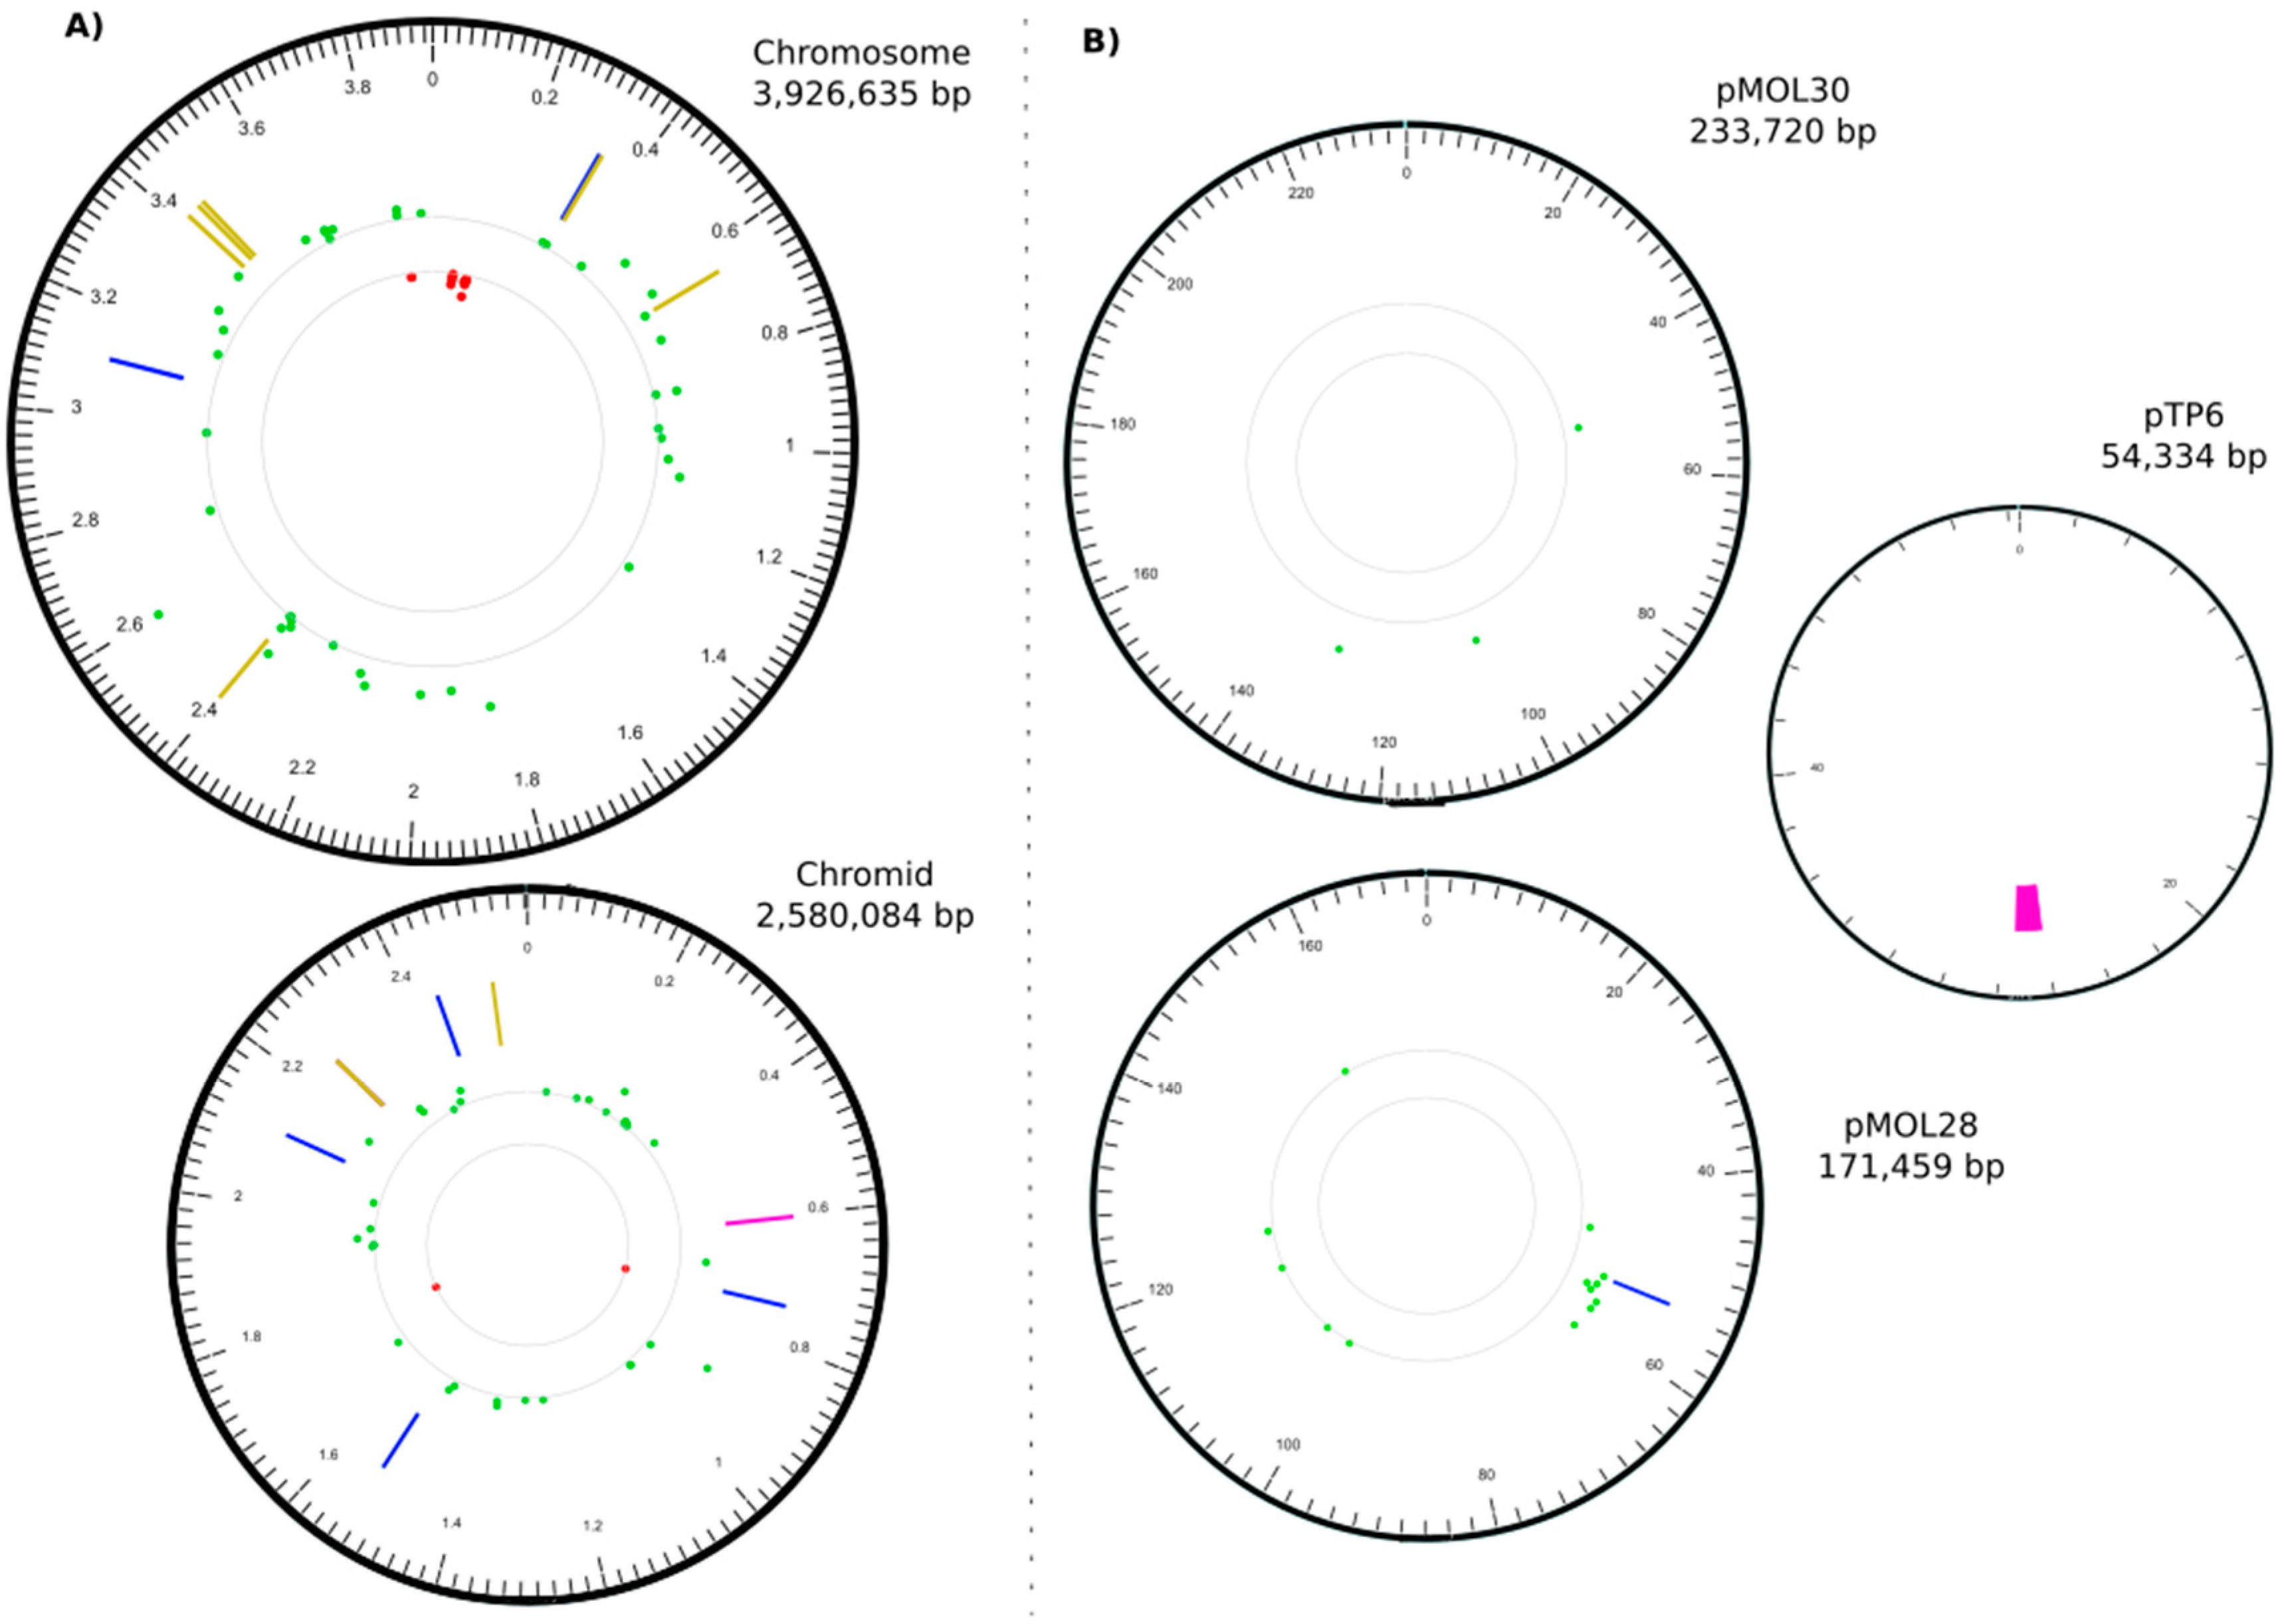
\includegraphics[width=\linewidth]{chapter3/chapter/figs/genes-09-00551-g001.png}
\end{center}
%\captionsetup{labelformat=empty}
\caption{Correlation map between Insertions or Deletions (INDELs), Single nucleotide polymorphisms (SNPs), and transcriptional changes found for \textit{C. metallidurans} MSR33. Concentric circles (ring) displayed from the outside inwards: (A) In ring 1, chromosome and chromid size scale in megabases (Mb) using a 20 kilobase (kb) window; (B) plasmids size scale in kb using a 2 kb window. In ring 2, position of insertion (blue), deletion (pink), and SNPs (mustard). INDELs and SNPs listed in Table \ref{table:42} and Table \ref{table:43}. In ring 3, each dot represents a single gene basal expression, overexpression (log$_2$ ratio $>$ 1, green), or repression (log$_2$ ratio $<$ -1, red), with a p-value $<$ 0.05. Circos plot created with Circa (http://omgenomics.com/circa).}
\label{chapter3-fig1}%
\end{figure*}


\begin{sidewaystable}
%\begin{table}[ht]
%\captionsetup{labelformat=empty}
\caption{Insertions (INs) and deletions (DELs) present in the genome of \textit{C. metallidurans} MSR33.\\}
\label{table:42}%
{%\hspace*{-4cm}
\begin{tabular*}{\columnwidth}{@{}llllllll@{}}
\hline
\textbf{Type} & \textbf{Replicon $^\#$} & \textbf{Start} & \textbf{End} & \textbf{Size (bp)} & \textbf{Description} & \textbf{Targeted} & \textbf{Function $^*$} \\
&  &  &  &  &  &  \textbf{Gene(s)}& \textbf{(MaGe Annotation)} \\
\hline
\\
IN & CHR1 &	328395 & 328395 & 1102 & IS1088 & Rmet\_0312 & Putative transporter \\
IN	& CHR1 & 3106728 & 3106728 & 1102 & IS1088 & Rmet\_2857 & Taurine ABC transporter \\
	&  &  &  &  &  &  (\textit{tauB}) &  ATP-binding protein\\
DEL &	CHR2 &	602035 &	602490 &	455	& &	Rmet\_4033 &	LysR family  \\
 &	 &	 &	 &		& &	& transcriptional regulator\\
IN &	CHR2 &	741818 &	741818 &	1102 &	IS1088 &	Rmet\_4160  &	EPS biosynthesis, \\
 &	 &	& &	 &	 & (\textit{pelF}) &	biofilm formation\\
IN &	CHR2 &	1529231 &	1529231 &	1102 &	IS1088 &	Rmet\_4867  &	Membrane fusion protein,\\
 &	 &	 &	 &	 &	 & (\textit{acrA}) &	multidrug efflux\\
IN &	CHR2 &	2113815 &	2113815 &	256 &	tniA/Tn3 &	Rmet\_5388  &	ApbE-like lipoprotein\\
 &	 &	 &	 &	 &	 &  (\textit{apbE}) & \\
IN &	CHR2 &	2253560 &	2253560 &	3 &	+CTT &	Rmet\_5508 &	Long-chain-fatty-acid\\
 &	 &	 &	 &	 & & & -CoA ligase\\
DEL &	CHR2 &	2253566 &	2253568 &	3 &	-CGG &	Rmet\_5508 &	Long-chain-fatty-acid\\
 &	 &	 &	 &	 & & & -CoA ligase\\
IN &	CHR2 &	2440975 &	2440975 &	1104 &	IS1088 &	Rmet\_5682 &	Membrane fusion protein, \\
 &	 &	 &	 &	 &	 &  (\textit{nimB})	& heavy metal transport\\
IN &	pMOL28 &	53484 &	53484 &	1104 &	IS1088 &	Rmet\_6205 &	Antisigma factor\\
DEL &	pTP6 &	26155 &	27385 &	1230 &	&	 (\textit{cnrY}),  &	Respectively an outer  \\
 &	 &	 &	 &	 &	& \textit{upf30.5}, & membrane protein, a \\
  &	 &	 &	 &	 &	& \textit{upf31.0}, &	DNA methylase, and \\
    &	 &	 &	 &	 &	& \textit{parA} &	a plasmid partition protein\\

\\
\hline
\hline
\end{tabular*}
} {\footnotesize{$^\#$ Chromosome: CHR1; chromid: CHR2. * Genomic and Metabolics analysis software (www.genoscope.cns.fr).} }
%\end{table}
\end{sidewaystable}

\begin{sidewaystable}
%\begin{table}[ht]
%\captionsetup{labelformat=empty}
\caption{ Single nucleotide polymorphisms (SNPs) detected in the genome of \textit{C. metallidurans} MSR33.\\}
\label{table:43}%
{%\hspace*{-4cm}
\begin{tabular*}{\columnwidth}{@{}llllll@{}}
\hline
\textbf{Replicon$^\#$} & \textbf{Position} & \textbf{SNP} & \textbf{SNP Type} & \textbf{Affected Gene} & \textbf{Gene Description$^*$} \\
\hline
CHR1 &	333850 & A→G & intergenic (+201/-75) &	Rmet\_0314 →/	& Putative transporter, major facilitator \\
 &	 &  &  & → \textit{ssb1}	& family/single-stranded DNA-binding \\
 &	 &  &  &	& protein (helix-destabilizing protein) \\
CHR1 &	645608	& A→G & A23A (GCA→GCG) &	Rmet\_0598  & Protein phosphatase family protein \\
 &	 &  &  & →	Ser/Thr	& \\
CHR1 &	2400725	& G→A	& intergenic (-77/+116) &	\textit{greA} ←/← \textit{carB} &	Transcription elongation factor/\\
&	 &  &  &	& carbamoyl-phosphate synthase large  \\
&	 &  &  &	& subunit  \\
CHR1 &	3418147	& A→G &	V295A (GTC→GCC) &	\textit{dppF} ←	& Dipeptide transporter; ATP-binding  \\
&	 &  &  &	& component of ABC superfamily \\
CHR1 &	3444412	& A→G &	V17A (GTC→GCC) &	\textit{nirJ} ← &	Heme d1 biosynthesis protein \\
CHR1 &	3456113 & A→G &	V76A (GTG→GCG) &	\textit{acyP} ← &	Acylphosphatase \\
CHR2 &	2253543 & A→T	& V158E (GTG→GAG) &	Rmet\_5508 ← &	Long-chain-fatty-acid-CoA ligase \\
CHR2 &	2253553 &	G→T	& P155T (CCG→ACG) &	Rmet\_5508 ← &	Long-chain-fatty-acid-CoA ligase \\
CHR2 &	2529357	& T→C &	G264G (GGA→GGG) & 	Rmet\_5769 ← & Esterase \\

\\
\hline
\hline
\end{tabular*}
} {\footnotesize{$^\#$ Chromosome: CHR1; chromid: CHR2; arrows show positive → or negative ← gene orientation; * www.genoscope.cns.fr.} }
%\end{table}
\end{sidewaystable}
The majority of the new IS1088 copies in the MSR33 genome were located on the chromosome and chromid, where all IS1088 copies indigenous to CH34 resided, but one IS1088 copy transposed into the \textit{cnrY} gene (Rmet\_6205) of pMOL28 (Table \ref{table:42}). This gene was part of the \textit{cnrYXHCBAT} locus involved in the inducible cobalt and nickel resistance in strain CH34, and encoded the anti-sigma factor CnrY that tethered, in conjunction with the sensor protein CnrX, the sigma factor CnrH, but released it in the presence of Ni$^{2+}$ or Co$^{2+}$ \citep{grass2000regulation, tibazarwa2000regulation}. The sigma factor CnrH promoted transcription of its own locus \textit{cnrYXH}, but also of the structural locus \textit{cnrCBA}, encoding a resistance nodulation division (RND)-driven efflux system \citep{janssen2010complete, kim2011switch}. The inactivation of the \textit{cnrY} gene in MSR33 by IS1088 inevitably led to the constitutive derepression of \textit{cnrCBAT} transcription and explained the increased cobalt and nickel resistance we observed for MSR33 (Table \ref{table:41}) (see also gene expression results in Section 3.3). A similar phenomenon was previously seen for spontaneous mutants of a pMOL30-less CH34 derivative, strain AE126 \citep{mergeay1985alcaligenes}, which showed a significantly increased resistance to cobalt and nickel \citep{collard1993new} and which was later acknowledged as being an IS- and frameshift-mediated inactivation of \textit{cnrY} and \textit{cnrX} \citep{vandecraen2016zinc}.
The other five genes affected by the insertion of an IS1088 element were Rmet\_0312 (\textit{nptA}) and Rmet\_2860 (\textit{tauB}), lying on the chromosome; and Rmet\_4160 (\textit{pelF}), Rmet\_4867 (\textit{acrA}), and Rmet\_5682 (\textit{nimB}), lying on the chromid (Table \ref{table:42}). The first three genes encode proteins with general cellular functions, and their inactivation is very unlikely to affect heavy metal resistance in strain MSR33. The fourth gene, \textit{acrA}, encodes a membrane fusion protein and is part of an intact \textit{acrABC} operon whose gene products form a tripartite multidrug efflux system. The last gene, \textit{nimB}, is involved in efflux-mediated heavy metal resistance, encoding also a membrane fusion protein resembling other membrane metal-binding fusion proteins in structure and function (e.g., CzcB, CnrB, CusB, and ZneB) by forming a periplasmic bridge between the cytoplasmic porter and the outer membrane channel \citep{kim2011switch}. Nonetheless, taking also into account that the \textit{nimA} gene is already inactivated in strain CH34 (and MSR33) by the presence of the insertion sequence element ISRme3 \citep{janssen2010complete}, it is hard to see how the inactivation of \textit{nimB} would result in the increased metal resistance we observed in strain MSR33. Two insertions were not attributed to IS1088. One appeared to be the result of a Tn3-related transposition event affecting gene Rmet\_5388, encoding a tentative ApbE-like lipoprotein, while the other concerned an unknown mutational event in gene Rmet\_5508 resulting in the insertion of a nucleotide triplet (+CTT) (Table \ref{table:42}). This gene encodes a long-chain fatty-acid CoA-ligase and also underwent a triplet deletion (-CGG) just a few nucleotides downstream of the triplet insert. As a combined result, the actual change at the protein level remained perfectly in-frame and gave a protein of the same length, but led to an altered peptide sequence at positions 149–153 (i.e., Xxx-Leu-Arg-Phe-Ala-Gln-Xxx in CH34 to Xxx-Leu-Phe-Ala-Lys-Gln-Xxx in MSR33 (amino acidic sequence change from Arg-Phe-Ala to Phe-Ala-Lys). The third deletion in MSR33 occurred in plasmid pTP6, effectively destroying the genes \textit{upf30.5}, \textit{upf31.0}, and \textit{parA}, immediately preceding Tn50580. Except for \textit{cnrY} and \textit{nimB}, none of the aforementioned genes are in any way associated with metal resistance.
In addition to the eight insertions and three deletions in the MSR33 genome, sequence analysis revealed the presence of nine single nucleotide polymorphisms (Table \ref{table:43}). Two of those occurred in intergenic regions on the chromosome, without apparent disruption of gene regulatory elements, while the other seven occurred in protein-encoding genes (four on the chromosome and three on the chromid). Except for the “silent” mutation (i.e., no \textit{aa} change) at position 645608, these Single nucleotide polymorphisms (SNPs) caused \textit{aa} substitutions in the corresponding gene products (Table \ref{table:43}). No SNPs were detected in any of the plasmids. Remarkably, gene Rmet\_5508 lying on the chromid (CHR2) once again was a target for mutation, displaying two SNPs in the immediate vicinity of the aforementioned triplet insertion and deletion in this gene (Table 3), bringing the full change of this region from RFAQKPAYV to FAKQKTAYE (changes are in bold and underlined). It is uncertain whether these protein changes would have any effect on the cellular and metabolic functions in MSR33.
Taken together, of the 11 Insertions or Deletions (INDELs) and nine SNPs identified by the whole genome resequencing of the \textit{C. metallidurans} strain MSR33, only the \textit{cnrY} inactivation by IS1088 and the concomitant derepression of \textit{cnrB} (see above) may be directly linked to the observed augmented heavy metal resistance in this strain, at least for Co$^{2+}$ and Ni$^{2+}$ (see above). None of the other genomic changes seemed to play a role in this augmentation. The augmented resistance for Cd$^{2+}$ in strain MSR33 (Table \ref{table:41}), however, remains a puzzle. The fact that such augmentation for Cd$^{2+}$ was only noted for MSR33 with an altered genome (i.e., with 17 INDELs and six SNPs), but not in CH34 transformed with plasmid pBBR::\textit{merTPAGB1} (Table \ref{table:41}) strongly indicates that the MSR33 genetic background was at play. In basic terms, bacterial resistance to toxic metals depends on two cellular processes, metal binding and metal transport, with the former generally being an intrinsic part of the latter. It is well established that many proteins or peptides that mediate the transport, buffering, or detoxification of metal ions in living cells have metal-binding domains (MBDs) in which certain amino acid residues (e.g., cysteine), as well as their structural layout and relative position to each other, play a key role in metal selectivity and specificity \citep{zheng2008data, thilakaraj2007silico}. While some of these proteins might be highly metal-specific, other proteins follow a more relaxed, nonspecific mode of metal binding. For instance, divalent metal uptake in \textit{C. metallidurans} is governed by a battery of redundant transporters that display a minimal degree of metal cation selectivity \citep{kirsten2011contributions}. Depending on the environment, this may lead to a cytoplasmic pool of unsolicited metal ions that at some point, particularly when reaching a toxic threshold, need to be removed by the cell. In \textit{C. metallidurans} this was done by one of three efflux systems: Cation diffusion facilitators (CDF), P-type ATPases, and the earlier mentioned RND-driven transenvelope transporters (HME-RND). Their main task in \textit{C. metallidurans}, because of this bacterium’s adaptation to metal-rich environments, was to balance the cytoplasmic and periplasmic concentrations of unwanted transition metals by entering the cellular arena and going into competition for metal cations with the “frivolous” metal uptake systems. Interestingly, all three types of metal efflux systems seemed to possess some degree of frivolity toward metal ions as well, albeit perhaps not as outspoken as for the metal uptake systems. The \textit{C. metallidurans} CzcD exporter (Rmet\_5979), for instance, allowed as a CDF protein Zn$^{2+}$, Cd$^{2+}$, or Co$^{2+}$ as a substrate \citep{anton1999czcd}, whereas the DmeF and FieF exporters (Rmet\_0198 and Rmet\_3406) displayed as CDF family members broad metal specificity for Zn$^{2+}$, Cd$^{2+}$, Co$^{2+}$, and Ni$^{2+}$ \citep{munkelt2004chromosomally}. It is worth mentioning that disruption of the \textit{dmeF} gene in strain CH34 dramatically lowered the resistance for Co$^{2+}$ (but not for Zn$^{2+}$, Cd$^{2+}$, and Ni$^{2+}$), indicating a complex interplay between the DmeF exporter and the CzcCBA and CnrCBA efflux pumps (possibly partially obscured by the action of other metal resistance systems) \citep{munkelt2004chromosomally}. Moreover, CDF proteins can play diverse roles and may possess different metal ion selectivity depending on the environmental conditions (i.e., by adjusted Kd values for certain metals) \citep{barber2017transition}. In addition, the eight metal resistance-related P1B-type ATPases currently identified in strain CH34 can be subdivided into two groups according to their substrate profile \citep{nies2016biological}: Those that extrude Cu$^+$ and Ag$^+$ (CupA and CupF) and those that extrude Zn$^{2+}$, Cd$^{2+}$, Co$^{2+}$, or Pb$^{2+}$ (ZntA, CadA, PbrA, and CzcP). These exporters mainly differ in the presence of unique amino acid sequences in their transmembrane MBDs, hence defining their metal specificity. But even within a subgroup, differences may exist in terms of metal affinity. For example, CzcP encoded by plasmid pMOL30 is unable to mediate Zn resistance on its own but rather augments the metal exportability of the ZntA, CadA, and PbrA exporters \citep{scherer2009czcp}. In a similar fashion, the five active HME-RND efflux systems in strain CH34 displayed a limited substrate spectrum, pumping out either the monovalent metal cations Cu$^+$ and Ag$^+$ (CusA, SilA) or the divalent metal cations Zn$^{2+}$, Ni$^{2+}$, and Co$^{2+}$, with occasionally also Cd$^{2+}$ (ZniA, CnrA, CzcA) \citep{nies2016biological} (Figure \ref{chapter3-fig2}). In such HME-RND systems, two steps of heavy-metal extrusion were discerned, the periplasmic and the transenvelope efflux (Figure \ref{chapter3-fig2}). Each step involved the interaction of metals with MBDs within the Membrane Fusion Protein (MFP) and RND proteins. Sometimes, the delivery of periplasmic metal ions to the typical C3B6A3-complex is facilitated by a small periplasmic metallochaperone, as is the case for the \textit{E. coli} CusCBFA system \citep{delmar2014bacterial} (and likely, based on CusF \textit{aa} sequence similarities, also the CusCBAF complex of strain CH34). Little is known about the substrate specificity of the metal-binding proteins of HME-RND efflux complexes. Apparently, metal-induced conformational changes in the C3B6A3-complex are required in order to create a proper metal-guiding C3B6A3 channel for metal export to take place \citep{kim2011switch,de2010metal,long2012structure,pak2013structures}.

\begin{figure*} [ht] 
\begin{center}
%\hspace*{-2.5cm}
\begin{subfigure}{0.48\textwidth}
    %\caption{Extracts and \textit{in vitro} experiment setup}
    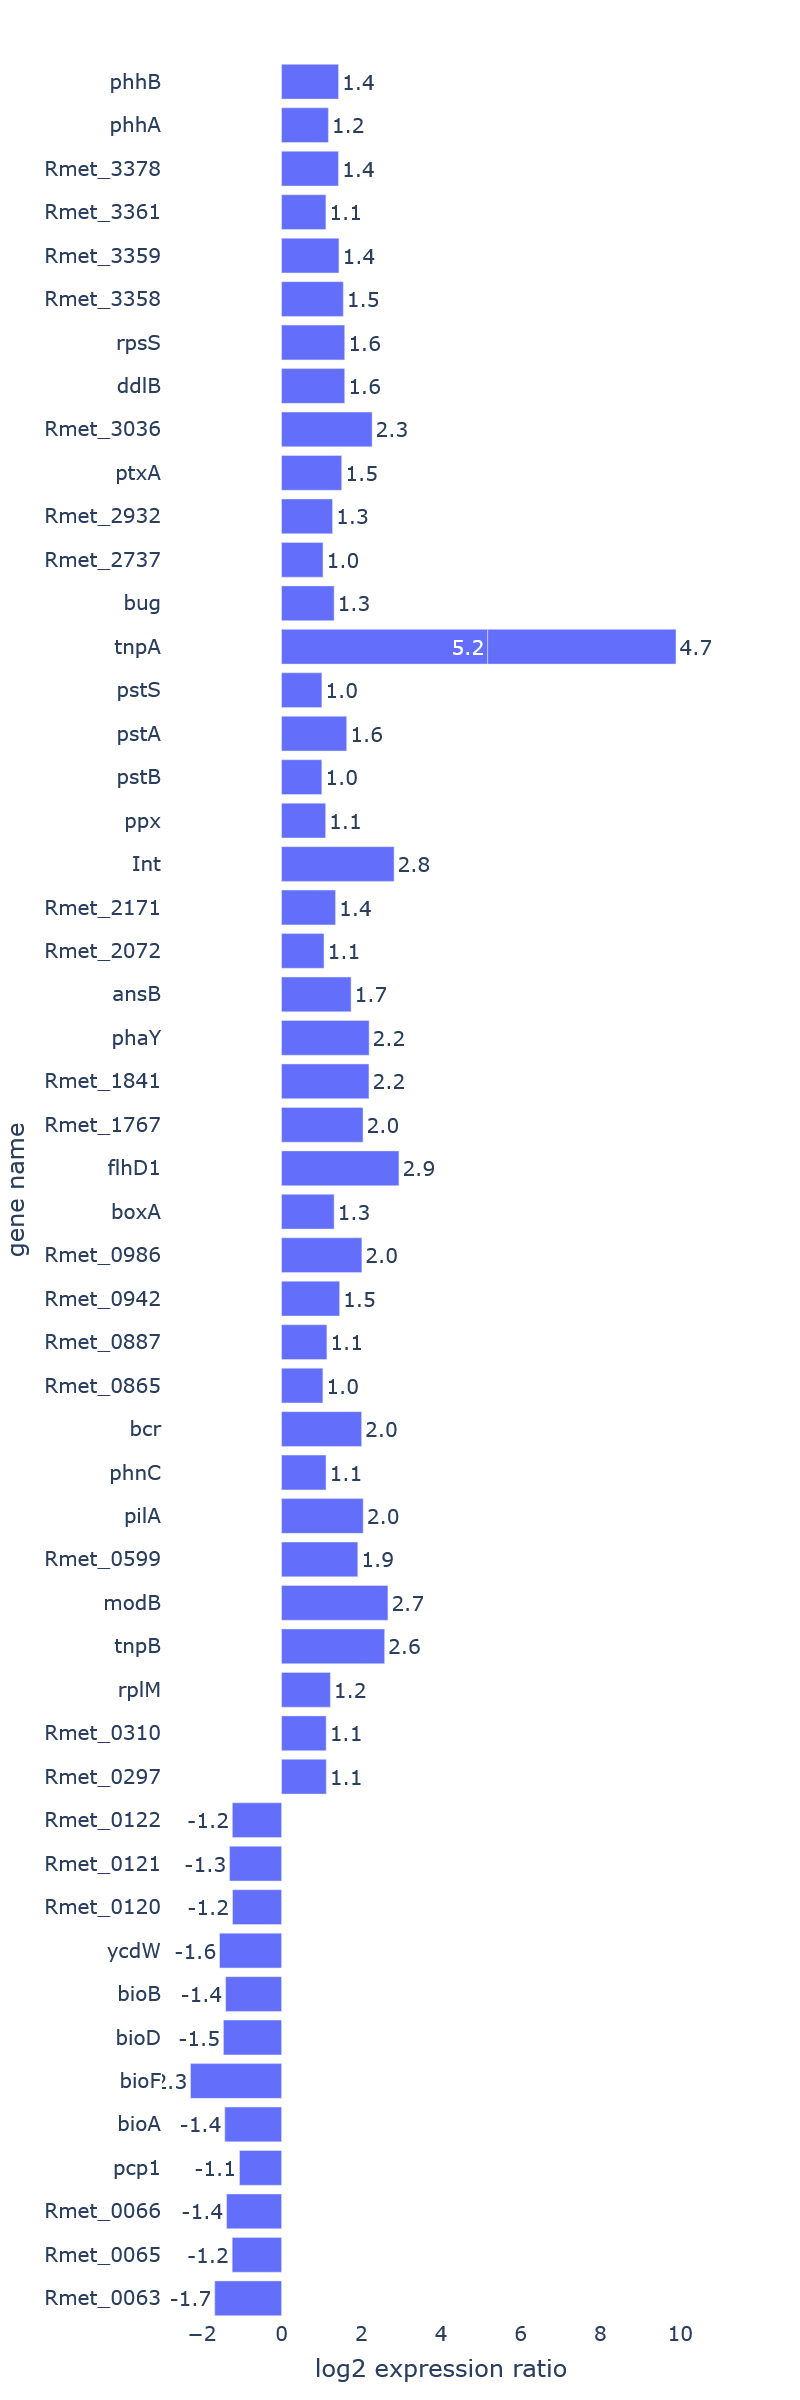
\includegraphics[width=\linewidth]{chapter3/chapter/figs/newplot(8).png}
     \label{fig:4a}
  \end{subfigure}
   \begin{subfigure}{0.48\textwidth}
    %\caption{Mytilid neutral red alive stain }
    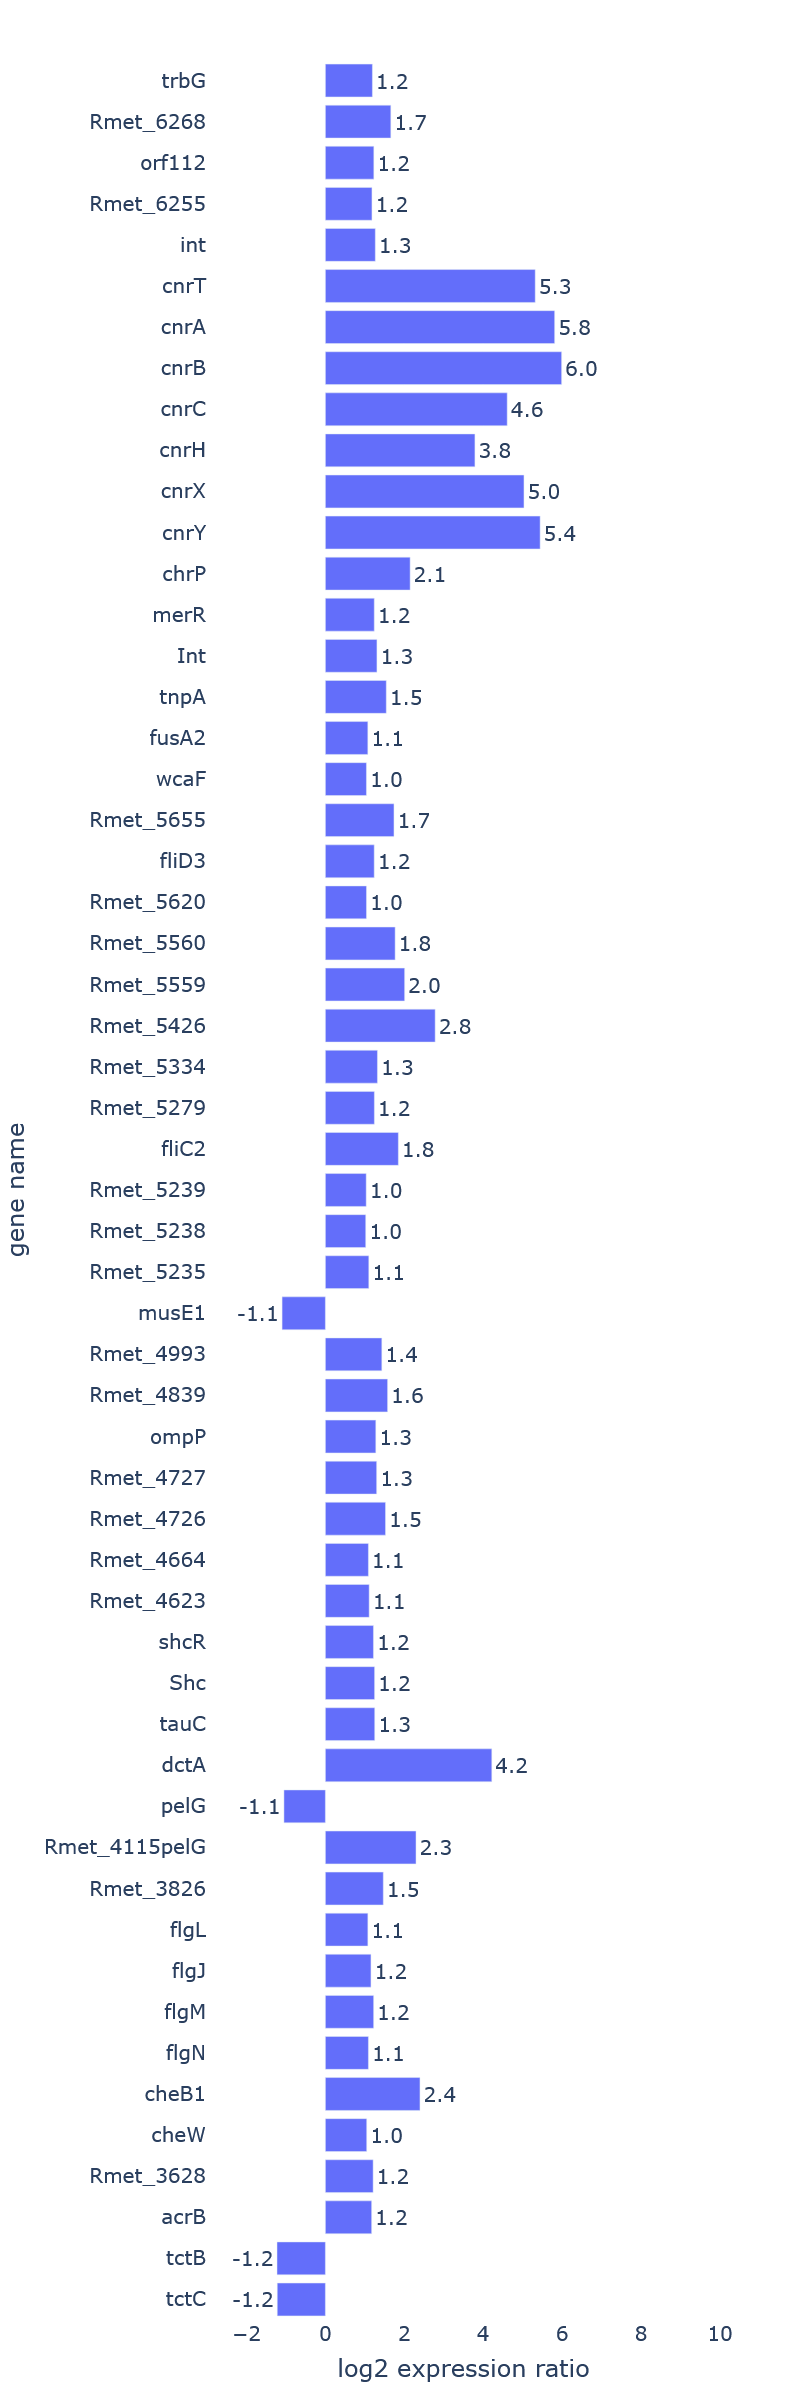
\includegraphics[width=\linewidth]{chapter3/chapter/figs/newplot(7).png}
     \label{fig:4b}
  \end{subfigure}
\end{center}
%\captionsetup{labelformat=empty}
\caption{Transcriptional changes in\textit{ C. metallidurans} MSR33 with respect to CH34, with both strains grown under equal and non-selective conditions (see methods). Bar graphs show the significantly (p-value $<$ 0.05) higher expression (log$_2$ ratio $>$ +1) and lower expression (log$_2$ ratio $<$ -1) of MSR33 genes (with CH34 gene expression levels as reference). 
}
\label{chapter3-fig2}%
\end{figure*}

\begin{figure*} [ht] 
\begin{center}
%\hspace*{-2.5cm}
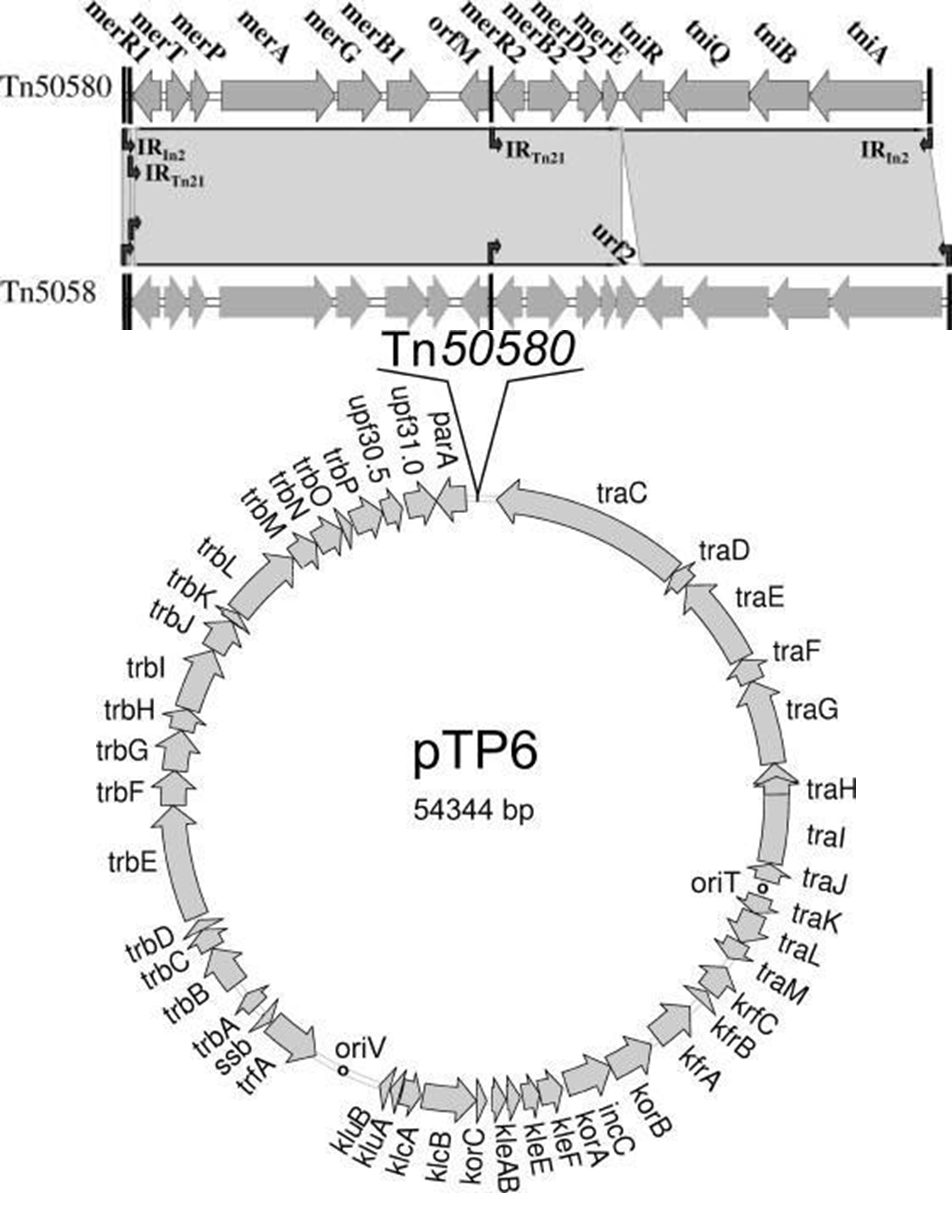
\includegraphics[width=300px]{chapter3/chapter/figs/genes-09-00551-g003.png}
\end{center}
%\captionsetup{labelformat=empty}
\caption{Genetic map of plasmid pTP6. Figure adapted from Smalla \textit{et al.}, 2006 (Copyright\textsuperscript{\tiny\textcopyright} 2006, Appl Environ Microbiol. 2006 Nov; 72(11): 7253–7259).   
}
\label{chapter3-fig3}%
\end{figure*}


As mentioned, it is not inconceivable that the genetic changes in MSR33 instigated cellular conditions or pleiotropic effects that were generally favourable for Cd$^{2+}$ detoxification and hence led to the observed improvement in Cd$^{2+}$ resistance. Possibly, this involved the temporal recruitment of one or more metal binding export proteins, from known metal resistant systems or from hitherto unknown export systems, able to bind Cd$^{2+}$. The transition metals cadmium and mercury belong to Group 12 of chemical elements in the periodic table, together with zinc and copernicium. Although these four metals differ in significant respects, they also have common properties. Particularly, Cd and Hg are similar in their outer shell electron configuration (d$^{10}$s$^2$) and atomic radius (ca. 150 pm), and their cations both have a high affinity for sulfhydryl groups in cellular compounds and proteins (i.e., in methionine and cysteine residues). From this perspective, competition between Cd$^{2+}$ and Hg$^{2+}$ for certain MBDs cannot be excluded. Bacterial evolution and adaptation to new or rapidly changing environments implies a delicate balance between the safeguarding of genome integrity and the tolerance for genome instability. A too-rigid genome inevitably will lead to the demise of innovative power and hence adaptability of the host, whereas a too plastic or “fluid” genome may lead to disadvantageous mutations and cell growth arrest, or even cell death. This balance between beneficiary and perilous change in a bacterial genome also relates to the general fitness and the energy household of its host. Members of the genus \textit{Cupriavidus}, and in particular \textit{C. metallidurans}, appear to be masters in adaptation as they are home to a wide variety of habitats, often in extreme conditions \citep{sota2007region,leys2009response,mijnendonckx2013characterization,byloos2017impact}. The introduction of the 54 kb plasmid pTP6 into a strain already carrying two large replicons of 3.9 and 2.6 Mb (chromosome and chromid, respectively) and two megasized plasmids of 171 and 234 kb (pMOL28 and pMOL30, respectively) could be seen as a serious additional burden to the host regardless of whether or not phenotypical or physiological changes occur.
Because the charting of genomic changes in MSR33 with respect to its parental strain CH34 did not provide us with any clues or direct evidence on the involvement of certain genetic loci or of any of the known metal resistance determinants on the observed augmented Cd$^{2+}$ resistance, we decided to compare the basal gene expression data for strains CH34 and MSR33 using RNA microarray technology in an attempt to associate their gene expression profiles with strain-specific physiological behaviour, with a focus on differentially expressed (DE) genes that might be involved in the cellular detoxification of heavy metals such as Cd$^{2+}$.

\subsection{Transcriptional Analysis of Strain MSR33}

Strains CH34 and MSR33, which were equally grown in nonselective conditions without any metal-related stress, were investigated for basal gene expression levels, and their expression profiles were compared. A total of 107 DE genes showed statistically significant changes in their expression (Figure \ref{chapter3-fig2}). Affected genes pertained to the main chromosome (55 genes), the chromid (36 genes), and the plasmids pMOL30 (3 genes) and pMOL28 (13 genes) (Figure \ref{chapter3-fig2}). In general terms, the products of these 107 genes could be grouped according to their predicted annotated function \citep{janssen2010complete}: Catalytic function (35 genes), transport (24 genes), transcriptional regulation (11 genes), recombination (6 genes), movement and chemotaxis (9 genes), and miscellaneous (22 genes). Most of these genes had a higher expression in strain MSR33, with only 16 genes in strain MSR33 showing a lower expression level. What is immediately striking is that all genes of the \textit{cnrYXHCBAT} operon on plasmid pMOL28 had a significantly higher expression (Figure \ref{chapter3-fig2}), with log$_2$ fold changes ranging from four to six. As we know from MSR33 whole genome sequence analysis, this high expression of the \textit{cnr} locus in strain MSR33 was the direct result of IS1088-mediated \textit{cnrY} inactivation and hence derepression of the \textit{cnr} locus, explaining the increased resistance we observed for strain MSR33 to Co$^{2+}$ and Ni$^{2+}$ (see previous sections). Equally noticeable is the complete absence of an altered expression of the \textit{czc} locus on pMOL30, strongly suggesting that the augmented Cd$^{+2}$ resistance we see for strain MSR33 was independent of this locus. This, in fact, corroborates earlier findings about the pMOL30-less CH34 derivative AE126 (which, like MSR33, also has an IS1088-mediated inactivated \textit{cnrY} gene on the remaining plasmid pMOL28):  \citet{vandecraen2016zinc} showed, next to a heightened resistance to Zn$^{2+}$, Co$^{2+}$, and Ni$^{2+}$, a 2-fold increased resistance to Cd$^{2+}$. Adding another level of complexity, when strains AE126 and AE104 (a CH34 derivative lacking both pMOL28 and pMOL30 plasmids \citep{mergeay1985alcaligenes}) were transformed with pTP6, these strains, like MSR33, gained an improvement in Cd$^{2+}$ resistance, albeit to a lesser extent (Rojas LA, personal communication).
This would indicate that the augmentation of Cd$^{2+}$ resistance in MSR33 by pTP6 conjugation should be seen as a layered process brought about by multiple factors and possibly diverse mechanisms supporting each other. We cannot say at this point what these mechanisms precisely are and how and when they are triggered, as we have no information about the genomic changes in pTP6 conjugants of AE104 and AE126 (as pTP6 conjugation in CH34 causes genomic changes, this would most likely also be the case for pTP6 conjugation in strains AE104 and AE126, but not necessarily involving the same genomic changes). Clearly, further studies are needed to understand the augmented metal resistance in pTP6 conjugants of CH34 and its derivatives, including (1) the resequencing of pTP6-conjugated AE104 and AE126 strains and (2) the extensive RNAseq-based genetic response analyses for a wider range of heavy metals in all three pTP6-conjugated strains. The additional possibility that some of the observed genetic changes were already introduced to the recipient CH34 strain prior to conjugation with pTP6 cannot be entirely excluded. Lastly, the plasmid-curing procedures used to obtain strains AE104 and AE126 (i.e., applying mitomycin C, nalidixic acid, or hydroxyurea to growing CH34 cells \citep{mergeay1985alcaligenes}) may also have had mutagenic effects or may have induced transposition activity. In this respect, it would be best, in the frame of future studies, to resequence these strains as well.
A very high log$_2$ fold difference in the expression of $>$4 was also noted in strain MSR33 for the Rmet\_4229 gene, a \textit{dctA} paralogue whose product was functionally annotated as a C4-dicarboxylate transporter and which is unlikely to have any connection to metal detoxification or resistance, and gene Rmet\_2382, originally identified in CH34 as a transposase-encoding \textit{tnpA} gene (IS1088) (Figure \ref{chapter3-fig2}). Intermediate high log$_2$ fold changes of $>$2 were seen in strain MSR33 for another 17 genes, whereas the remaining 72 genes showed a log$_2$ fold change between one and two. None of these genes is thought to be involved in metal binding, metal detoxification, or metal resistance. Among the genes with lowered expression in strain MSR33, we noted the \textit{pelG} gene (Rmet\_4161), which is part of the \textit{pelABCDEFG} operon required to produce an extracellular polysaccharide that has been implicated in biofilm development \citep{vasseur2005pel}. Our sequence data confirmed that the IS1088 element transposed into the \textit{pelF} gene (Table \ref{table:42}), thereby disrupting expression of the \textit{pelG} gene. This could explain the complete lack of biofilm formation in strain MSR33 reported to us by P. Alviz in a personal communication.
In conclusion, the genome of MSR33 underwent eight insertions, three deletions, and nine SNPs. At least seven of the insertions were due to the action of mobile genetic elements, with their presence fully confirmed by sequence data (implicating IS1088 in six cases), whereas one small insertion and all three deletions in strain MSR33 may have been the result of DNA recombination or transposition events. The \textit{C. metallidurans} genome is known to be ridden with a very high number of mobile genetic elements, with 57 IS elements, 19 other transposable elements, and 16 genomic islands for its type strain CH34 \citep{janssen2010complete,van2009new,van2012variation}. In concordance with this genomic fluidity, \textit{C. metallidurans} displays a highly versatile metabolism and an inherent ability to inhabit a variety of harsh environments \citep{sobecky2009horizontal,sota2007region,leys2009response,mijnendonckx2013characterization,byloos2017impact}. This adaptability has not come about overnight but is the wonderful result of microbial evolution over long periods of time. In a time in which large chunks of DNA were retrieved from the environment (e.g., by plasmid transfer or gene exchanges), adaptation was brought about by DNA mutations and natural selection and molecular inventions took place, steadily moulding the genome into its present large (6.9 Mb) and highly malleable form, providing the bacterium with a vast array of possibilities for rapid genetic responses (hence its well-chosen epithet as “Master Survivalist”) \citep{janssen2010complete}. However, tinkering with this hugely evolved and dynamic genome holds intrinsic dangers. Although the plasmid pTP6 was maintained stably in strain CH34 (i.e., MSR33) for over 70 generations under nonselective conditions \citep{rojas2011characterization}, it has now become clear from our study at hand that the receiving host’s genome underwent multiple changes in the form of 11 INDELs and 9 SNPs, affecting the physiology and heavy metal resistance of the host. It would be wrong to point the finger at the extra plasmid as the “usual suspect” for these genetic changes, but rather we hold the actual process of conjugation responsible. Conjugative interaction appears to be a strong stimulus for transposition \citep{godoy2000transposon,christie2009conjugative,baharoglu2010conjugative}, and hence it is easy to envisage that, as a result of conjugation procedures, some elements of the extensive mobilome of \textit{C. metallidurans} (with nearly 100 mobile elements) were triggered into action and “moved around”, causing genetic changes that led to clearly perceptible but also less visible (and less understood) effects alike. The take-home message here is that the genetic engineering of bacteria with large complex and dynamic genomes should be carried out with much caution and that a strong preference should be given to the new generation of small broad-host-range cloning vectors and CRISPR-based technologies nowadays available \citep{jain2013broad,obranic2013improvement,tian2017fundamental,cook2018genetic,xiong2018genome}.

\begin{figure*} [ht] 
\begin{center}
\hspace*{-1.5cm}
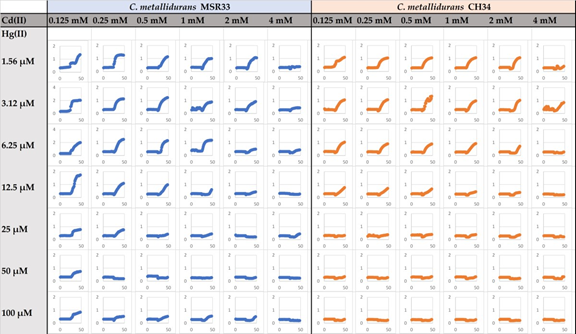
\includegraphics[width=500px]{chapter3/chapter/figs/genes-09-00551-g004.png}
\end{center}
%\captionsetup{labelformat=empty}
\caption{Effect of various mixtures of Hg$^{2+}$ and Cd$^{2+}$  on \textit{C. metallidurans} strains MSR33 and CH34 growth.   
}
\label{chapter3-fig4}%
\end{figure*}

\section{Supplementary Materials}

The following are available online at https://www.mdpi.com/2073-4425/9/11/551/s1. Figure S1: Genetic map of plasmid pTP6; Table \ref{table:44}: Primers designed for this report; Table \ref{table:45}: Transcriptional changes observed in MSR33 versus CH34 under basal conditions; Table \ref{table:46}: Homology analysis of \textit{mer} gene products present in plasmid pTP6; Figure \ref{chapter3-fig4}: Effect of various mixtures of Hg$^{2+}$ and Cd$^{2+}$ on \textit{C. metallidurans} strains MSR33 and CH34 growth; Table \ref{table:47}: Plasmid copy number (PCN) for \textit{C. metallidurans} strains MSR33 and CH34, determined by quantitative PCR; Table \ref{table:48}: mer gene occurrences on the replicons of strains CH34 and MSR33.

\section{Author Contributions}

F.A.M., P.J.J., R.V.H., P.M., and L.A.R. conceived and designed the experiments; F.A.M., A.J., and A.P. performed the experiments; F.A.M., R.V.H., and P.M. analyzed the data; L.A.R. and P.J.J. contributed reagents, materials, and analysis tools; F.A.M., P.J.J., R.V.H., P.M., and L.A.R. wrote the paper.
Funding
SCK$\cdot$CEN EE0630012-09 (to P.J.J., R.V.H., A.J., A.P., and P.M.), CONICYT/FONDECYT 11130117 (L.A.R.), and CONICYT/BC-PhD 72170403 (F.A.M.)

\section{Acknowledgments}
Authors acknowledge research funding by SCK$\cdot$CEN EE0630012-09 (to P.J.J., R.V.H., A.J., A.P., and P.M.), CONICYT/FONDECYT 11130117 (L.A.R.), and CONICYT/BC-PhD 72170403 (F.A.M.). Genome sequencing was provided by MicrobesNG (http://www.microbesng.uk), supported by BBSRC grant number BB/L024209/1. We thank D. Vallenet and Z. Rouy of Génoscope (Centre National de Séquençage, Evry, France) for implementing additional features in MaGe and their essential advice in genome annotation.

\section{Conflicts of Interest}
The authors declare no conflicts of interest. The founding sponsors had no role in the design of the study; in the collection, analyses, or interpretation of data; in the writing of the manuscript; or in the decision to publish the results.


\begin{sidewaystable}[ht]
%\captionsetup{labelformat=empty}
\caption{Primers used in this study.\\}
\label{table:44}%
{%\hspace*{-5cm}
\begin{tabular*}{\columnwidth}{@{}lllll@{}}
\hline
\textbf{Targeted gene} & \textbf{Replicon} & \textbf{Primer} & \textbf{Sequence (5'-3')} \\
\hline
\textit{merTPAGB1} & pTP6 & pTP6mer\_Fw & CACTATAGGGCGAATTACGGTCTTTTCTGACGTTGG\\
& & pTP6mer\_Rv & AAGGGAACAAAAGCTGTTCTAGCCACTTTCGGTTCG\\
MCS & pBBR1 & pBBR1MCS2\_GA\_Fw & CAGCTTTTGTTCCCTTTAGTGAG\\
 &  & pBBR1MCS2\_GA\_Rv & AATTCGCCCTATAGTGAGTCGTAT\\
\textit{cadA} & Chromosome & CadA\_Fw\_CR1 & GCACACTCACACATGGCAAG\\
 &  & CadA\_Rv\_CR1 & CTGAGACACAGGATGGTCCG\\
\textit{zniA} & Chromid  & ZniA\_Fw\_CR2 & GCGCAGATCACCCAGGAATA\\
 &  & ZniA\_Rv\_CR2 & ACTATGACCGTTCGACGCTG\\
\textit{nccA} & pMOL30 & NccA\_Fw\_P30 & AAGAGTGAATGGCCGGATGG\\
 &  & NccA\_Rv\_P30 & TCTCAATGGGTTGGGTGACG\\
 \textit{cnrA} & pMOL28 & CnrA\_Fw\_P30 & AAATGTCCCGATCACAGTCGG\\
 &  & CnrA\_Rv\_P30 & GCCCACCACCGTTTCATTG\\
  \textit{merG} & pTP6 & MerG\_Fw\_PT6 & TACAAATGCGGTATGGGCGT\\
 &  & pTP6\_Rv\_PT6 & CGAGGTTGAACTGTGCATCG\\
\\
\hline
\hline
\end{tabular*}
}
\\
{
%\footnotesize{}
}
\end{sidewaystable}


\begin{table}[ht]
%\captionsetup{labelformat=empty}
\caption{Transcriptional changes in MSR33 vs CH34 under equal, non-selective conditions.\\}
\label{table:45}%
{%\hspace*{-5cm}
\begin{tabular*}{\columnwidth}{@{}lll@{}}
\hline
 & \textbf{No genes} & \textbf{\%Total} \\
\hline
Total genes & 6099 & 100\\
Pval $>$0.05 & 5462 & 89.56\\
Pval $<$0.05 & 637 & 10.44\\
Overexpressed (log$_2$ $>$1) & 87 & 0.014\\
Repressed (log$_2$ $<$-1) & 15 & 0.002\\
Highly overexpressed (log$_2$ $>$2) & 27 & 0.004\\
Highly repressed (log$_2$ $<$-2) & 1 & 0.001\\
\\
\hline
\hline
\end{tabular*}
}
\\
{
%\footnotesize{}
}
\end{table}



\begin{sidewaystable}[ht]
%\captionsetup{labelformat=empty}
\caption{Sequence similarity of \textit{mer} gene products present in plasmid pTP6.\\}
\label{table:46}%
{%\hspace*{-5cm}
\begin{tabular*}{\columnwidth}{@{}lllll@{}}
\hline
 \textbf{Gene} & \textbf{Protein (aa)} & \textbf{Function} & \textbf{Organism (Reference)} & \textbf{\%ID (aa)}\\
 \hline
 \textit{merR1} & MerR (144) & activator/repressor of \textit{mer} operon & \textit{C. metallidurans} CH34 & 95\% (144) \\
  &  &  &  (YP\_145639.1) &  \\
 \textit{merT} & MerT (116) & mercuric ion transport protein & \textit{C. metallidurans} CH34  & 87\% (116) \\ 
   &  &  &  (YP\_145638.1) &  \\
 \textit{merP} & MerP (91) & periplasmic mercuric-ion binding protein & \textit{C. metallidurans} CH34  & 77\% (91) \\
    &  &  &  (YP\_145637.1) &  \\
 \textit{merA} & MerA (569) & mercuric-ion reductase Fad flavoprotein & \textit{C. metallidurans} CH34  & 71\% (561) \\ 
     &  &  &  (YP\_145636.1) &  \\
 \textit{merG}* & MerG (217) & organomercurial transporter & \textit{C. testosterone} JL40  & 100\% (190) \\ 
     &  &  &  (KGH30768.1) &  \\
 \textit{merB-}1* & MerB(212) & organomercurial lyase & \textit{B. cepacia} 2a  & 100\% (212) \\
    &  &  &  (YP\_006965881.1) &  \\
\textit{merR}2 & MerR (144) &
activator/repressor of \textit{mer} operon & \textit{C. metallidurans} CH34  & 93\% (144)\\
&&&(YP\_145639.1)&\\
\textit{merB}-2* & MerB (212) & organomercurial lyase & \textit{B. cepacia} 2a  & 100\% (212) \\
    &  &  &  (YP\_006965883.1) &  \\
\textit{merD} & MerD (121) & secondary regulatory protein & \textit{C. metallidurans} CH34  & 92\% (121) \\
    &  &  &   (YP\_145635.1) &  \\
\textit{merE} & MerE (78) & membrane mercuric resistance protein & \textit{C. metallidurans} CH34   & 79\% (78)\\
    &  &  &  (YP\_145634.1) &  \\
\\
\hline
\hline
\end{tabular*}
}
\\
{
\footnotesize{*Genes not present in \textit{C. metallidurans} CH34}
}
\end{sidewaystable}

\begin{sidewaystable}[ht]
%\captionsetup{labelformat=empty}
\caption{Plasmid copy number (PCN) for \textit{C. metallidurans} strains MSR33 and CH34.\\}
\label{table:47}%
{%\hspace*{-5cm}
\begin{tabular*}{\columnwidth}{@{}llllllllll@{}}
\hline
 \textbf{Replicon} & \textbf{Ct} & \textbf{SD} & \textbf{Log$_{10}$(DNA)} & \textbf{PCN}  & \textbf{Ct} & \textbf{SD} & \textbf{Log$_{10}$(DNA)} & \textbf{PCN} & \textbf{Average PCN}\\
 \hline
Chromosome (\textit{cadA}) & 23.38 & 0.05 & 10.18 & 1.00 & 23.47 & 0.21 & 10.18 & 1.00  & 1.00\\
Chromid (\textit{zniA}) & 20.90 & 0.19 & 10.24 & 1.16 & 20.18 & 0.07 & 10.24 & 1.14  & 1.15\\
pMOL30 (\textit{nccA}) & 21.71 & 0.29 & 10.26 & 1.21 & 19.75 & 0.20 & 10.24 & 1.14  & 1.18\\
pMOL28 (\textit{cnrA}) & 27.80 & 0.24 & 10.25 & 1.18 & 24.62 & 0.07 & 10.23 & 1.12  & 1.15\\
pTP6 (\textit{merG})* & 20.67 & 0.08 & 10.50 & 1.81 & 35.28 & 0.60 & 9.48 & 0.17  & 0.99\\
\\
\hline
\hline
\end{tabular*}
}
\\
{
\footnotesize{*Gene not present in \textit{C. metallidurans} CH34}
}
\end{sidewaystable}

\begin{table}[ht]
%\captionsetup{labelformat=empty}
\caption{\textit{mer} gene  occurrence  on  replicons  of  strains  CH34  and  MSR33  (individual  genes  of  the \textit{merRT}, \textit{merRTPA}, \textit{merRDE}, \textit{merRTPA} or \textit{merRTPADE} loci are indicated).\\}
\label{table:48}%
{%\hspace*{-5cm}
\begin{tabular*}{\columnwidth}{@{}llllllll@{}}
\hline
 \textbf{Replicon} & \multicolumn{6}{c}{\textbf{\textit{mer} genes present on each replicon }} & \textbf{PCN*} \\
 \hline
CHR1 & R & T & P & A &   &   & 1.00\\
pMOL28 & R & T & P & A & D & E & 1.15\\
pMOL30 - cluster 1 & R & T & P & A & D & E & 1.18\\
pMOL30 - cluster 2 & R & T & P & A & D & E & 1.18\\
Strain CH34 & 4.51 & 4.51 & 3.33 & 3.33 & 2.33 & 2.33 & \\
pTP6 - cluster 1 & R & T & P & A &  &  & 1.8\\
pTP6 - cluster 2 & R &  &  &  & D & E & 1.8\\
Strain MSR33 & 8.11 & 6.31 & 5.13 & 5.13 & 4.13 & 4.13 & \\
Gene unit increase & +2 & +1 & +1 & +1 & +1 & +1 & \\
Gene content increase & 80\% & 40\% & 54\% & 54\% & 77\% & 77\% & \\
\\
\hline
\hline
\end{tabular*}
}
\\
{
\footnotesize{*PCN values were taken from Table \ref{table:47}}
}
\end{table}